\chapter{Results}
In this chapter, various mobile subscriber trajectories will be presented that have been generated using the developed system. Mobile subscription data from several subscribers captured by the OpenCoverageMap was used. The generated trajectories cover rural and urban areas, which allows evaluating the approach for several scenarios. All results are fully reproducible in case the same subscriber and coverage predictions are used.
\section{Example 1}
The first example covers a semi-rural region. A semi-rural region consist of a rural and an urban area. The following trajectory was recorded on Monday, 26 March 2012. At 08:08:29 in the morning\  the subscriber established a call. The duration of the call was 7 minutes and 36 seconds.  During the call the subscriber traversed the highway A7 from Linz\footnote{GPS position of call establishment Latitude: 48.28086955 Longitude:	14.30415398 \url{http://osm.org/go/0JhMzsg9l-?m=}} to Engerwitzdorf\footnote{GPS position of call termination Latitude: 48.3381025 Longitude:	14.4125565 \url{http://osm.org/go/0JhP~5vT--?m=}}. Between the call establishment and call termination the mobile station was connected to 22 transmitters which resulted in 21 handover events. Figure~\ref{fig:563overview} illustrates the traversed route as well as the estimated handover position for both the network planning tool coverage~\ref{fig:563coverage} and the Voronoi diagrams coverage~\ref{fig:563voronoi}.

%\begin{figure}
%\begin{tabular}{cc}
%  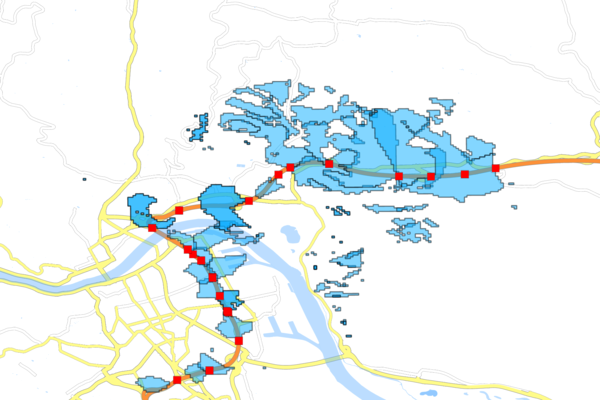
\includegraphics[width=65mm]{./images/563_Coverage_Handover} 
%  &   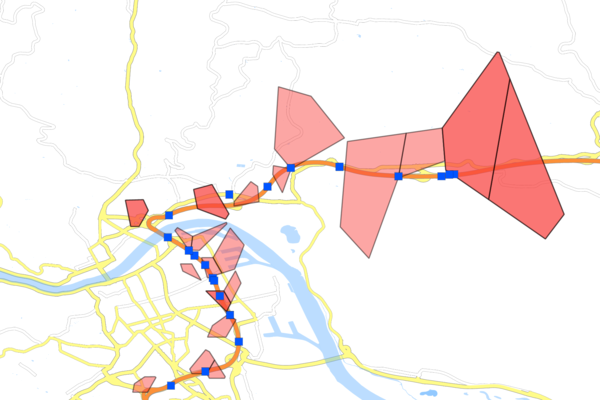
\includegraphics[width=65mm]{./images/563_Voronoi_Handover} \\
%(a)  & (b)  \\[6pt]
% 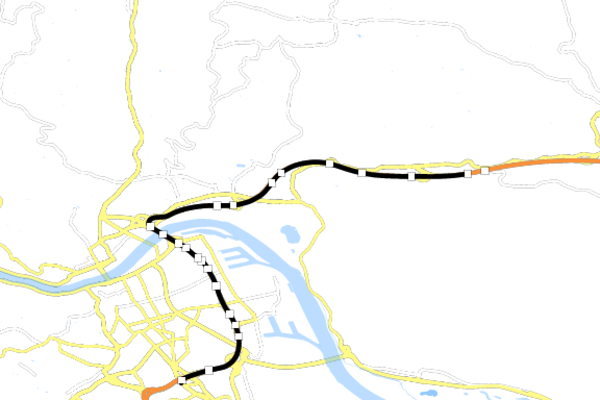
\includegraphics[width=65mm]{./images/563_Handover} 
% &   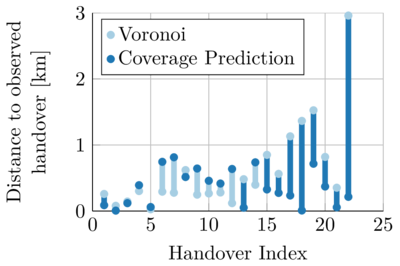
\includegraphics[width=65mm]{./images/563_predvorcomp} \\
%(c)  & (d)  \\[6pt]
%\end{tabular}
%\caption{Example 1 subscriber 563: (a) coverage prediction with network planning tool and estimated handover points, (b) Voronoi diagram coverage and estimated handover points, (c) recorded GPS route and observed handover points, (d) comparison of distance between estimated handover and observed handover}
%\label{fig:563overview}
%\end{figure}



\begin{figure}
	\centering
	\begin{subfigure}[b]{0.5\linewidth}
		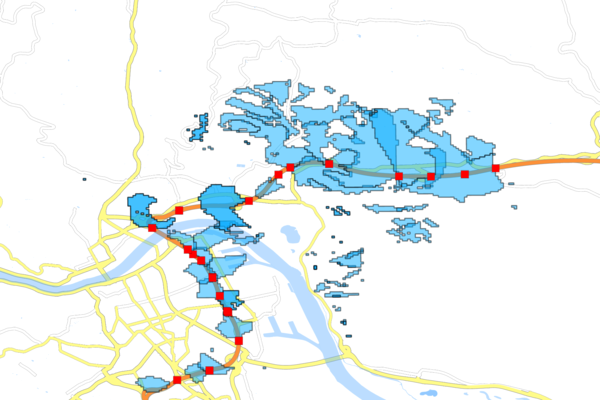
\includegraphics[width=\textwidth]{./images/563_Coverage_Handover}
		\caption{}
		\label{fig:563coverage}
	\end{subfigure}%
	~
	 %add desired spacing between images, e. g. ~, \quad, \qquad etc.
	%(or a blank line to force the subfigure onto a new line)
	\begin{subfigure}[b]{0.5\linewidth}
		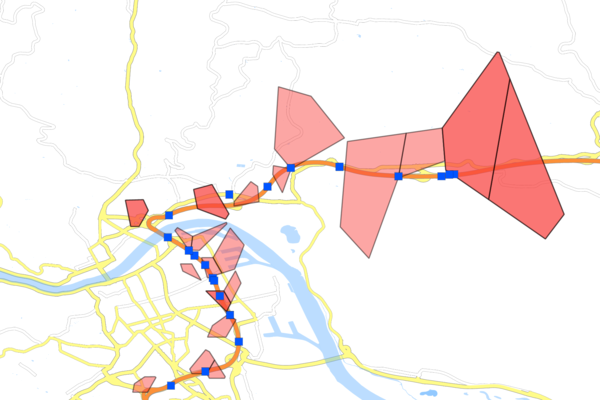
\includegraphics[width=\textwidth]{./images/563_Voronoi_Handover}
		\caption{}
		\label{fig:563voronoi}
	\end{subfigure}
	
	\begin{subfigure}[b]{0.5\linewidth}
			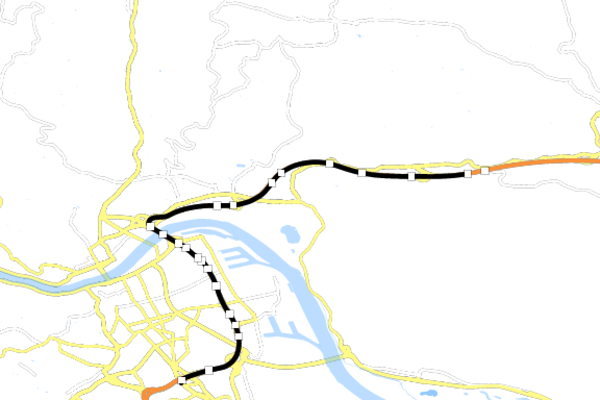
\includegraphics[width=\textwidth]{./images/563_Handover}
			\caption{}
			\label{fig:563handover}
		\end{subfigure}%
		~
		 %add desired spacing between images, e. g. ~, \quad, \qquad etc.
		%(or a blank line to force the subfigure onto a new line)
		\begin{subfigure}[b]{0.5\linewidth}
			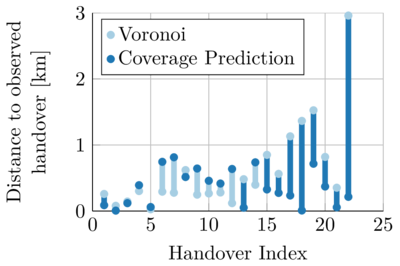
\includegraphics[width=\textwidth]{./images/563_predvorcomp}
			\caption{}
			\label{fig:563distcomp}
		\end{subfigure}
	
	\caption{Example 1 subscriber 563: (a) coverage prediction with network planning tool and estimated handover points, (b) Voronoi diagram coverage and estimated handover points, (c) recorded GPS route and observed handover points, (d) comparison of distance between estimated handover and observed handover}\label{fig:563overview}
\end{figure}


\subsection{Route}
To estimate the subscribers route, 20 random start and end positions within the coverage area of the first and last cell were used. The random positions were derived from a probability density function that was generated by the population density in the area as described in Section~\ref{sec:startandend}. Table~\ref{tab:563route} depicts the metrics used to choose the best approximation. The time-ration in conjunction with the squared sum of distances between the route and each coverage area allows the system to choose the best approximated route. In case of subscriber 563 the route with time-ration $1.00$ and $\sum {d}_{i}^{2}=0.35$ was picked. To compare the estimated route with the real route recorded with GPS the Hausdorff metric was used. The Hausdorff metric for the chosen route  compared with the actual route was $0.990138 $. That means that maximum distance between the chosen route and the actual route was very small. Thus, the similarity of  both routes is high. A second metric which takes the continuity of both routes into account is the Frechet distance. A Frechet distance of $0$ means that both routes are identical. Therefore, the smaller the Frechet distance is, the higher is the similarity. The computed Frechet distance for the estimated route is $0.0134$. Even if the estimated route corresponds to the actual route -- recorded with GPS -- there is a Frechet distance $>0$. This is due to the fact that GPS introduces an error which can lead to a deviation.

\begin{table}
\centering
\begin{tabular}{l|l|l|l}
Time-ratio & Mean distance $\overline{d_i}$ & Variance $\mathrm{Var}[d_i]$& $\sum {d}_{i}^{2}$ \\
\hline
0.96 & 0.09 & 0.03 & 1.38 \\
0.97 & 0.04 & 0.01 & 0.36 \\
0.97 & 0.09 & 0.03 & 1.39 \\
0.99 & 0.04 & 0.01 & 0.35 \\
0.99 & 0.04 & 0.01 & 0.35 \\
0.99 & 0.09 & 0.03 & 1.38 \\
\textbf{1.00} & \textbf{0.04 }& \textbf{0.01} & \textbf{0.35} \\
1.00 & 0.04 & 0.01 & 0.35 \\
1.01 & 0.05 & 0.01 & 0.42 \\
1.01 & 0.09 & 0.03 & 1.38 \\
1.02 & 0.04 & 0.01 & 0.36 \\
1.03 & 0.09 & 0.03 & 1.38 \\
1.03 & 0.09 & 0.03 & 1.38 \\
1.04 & 0.04 & 0.01 & 0.36 \\
1.04 & 0.09 & 0.03 & 1.38 \\
1.05 & 0.04 & 0.01 & 0.35 \\
1.05 & 0.09 & 0.03 & 1.38 \\
1.08 & 0.07 & 0.03 & 1.18 \\
1.10 & 0.07 & 0.03 & 1.18 \\
1.10 & 0.07 & 0.03 & 1.18
\end{tabular}
\caption{Comparison of 20 generate route with different start and end positions}
\label{tab:563route}
\end{table}
\subsection{Handover}
After an approximation of the subscriber has been chosen handover points were estimated. The estimation was done for both the network coverage prediction and the Voronoi diagram coverage. Figure~\ref{fig:563distcomp} shows a comparison of distances between the observed handover position and the estimated handover position for both coverage predictions. It can be seen that the handover estimation done with Voronoi diagram coverage performed better than the network coverage prediction for the first half of the route. On the other hand the network coverage prediction performed better in the second half of the route. 
\subsection{Velocity}
The velocity for each segment has been calculated with the approach introduced in Section~\ref{sec:velocity}.
\begin{figure}
	\centering
	\begin{subfigure}[b]{\textwidth}
		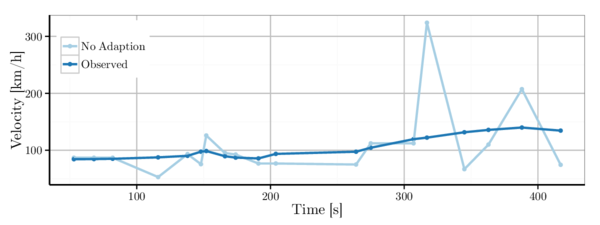
\includegraphics[width=\textwidth]{./images/563_velocityNoAdapt}
		\caption{}
		\label{fig:disthandover}
	\end{subfigure}%
	
	 %add desired spacing between images, e. g. ~, \quad, \qquad etc.
	%(or a blank line to force the subfigure onto a new line)
	\begin{subfigure}[b]{\textwidth}
		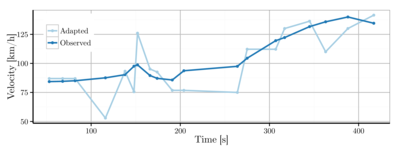
\includegraphics[width=\textwidth]{./images/563_velocityAdapt}
		\caption{}
		\label{fig:distmoc}
	\end{subfigure}
	\caption{Comparison of velocity (a) without adaption  and (b) with adaption}\label{fig:563velocity}
\end{figure}

\section{Example 2}

\section{Timing Information}
\subsection{Semi-Rural Trajectory}


\subsection{Urban Trajectory} 
Two trajectories in urban areas are presented. The first trajectory is generated for a subscriber in Linz, Austria whereas the second is generated for a subscriber in Vienna, Austria. Both trajectories are generated with Voronoi diagrams and Network Coverage Predictions.
\subsubsection{Example 1 - Subscriber 1058}
This subscriber traveled first on the minor road network in Linz and later used the highway A7.

\begin{figure}
\begin{tabular}{cc}
  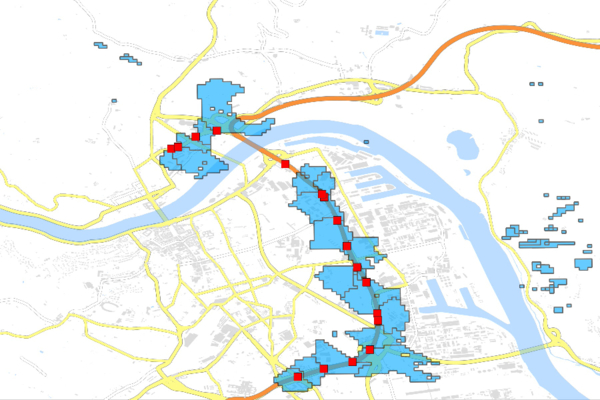
\includegraphics[width=65mm]{./images/1058_Coverage_Handover} 
  &   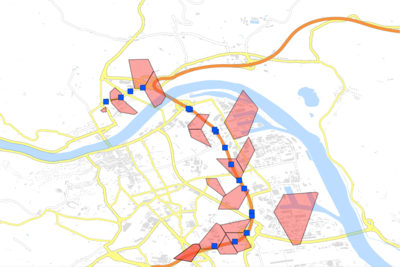
\includegraphics[width=65mm]{./images/1058_Voronoi_Handover} \\
(a) first & (b) second \\[6pt]
 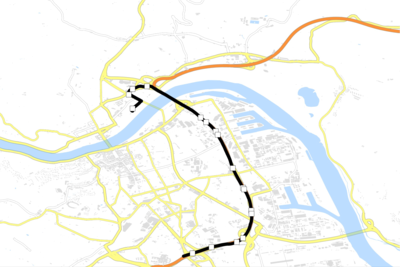
\includegraphics[width=65mm]{./images/1058_Handover} 
 &   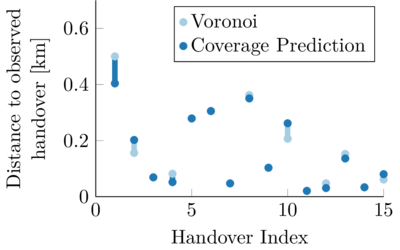
\includegraphics[width=65mm]{./images/1058_predvorcomp} \\
(c) third & (d) fourth \\[6pt]
\end{tabular}
\caption{Example 1 subscriber 1058: (a) coverage prediction with network planning tool and estimated handover points, (b) Voronoi diagram coverage and estimated handover points, (c) recorded GPS route and observed handover points, (d) comparison of distance between estimated handover and observed handover}
\label{fig:tettaroutes}
\end{figure}

\subsubsection{Example 2 - Subscriber }
\section{Coverage Prediction Difference}
\subsection{Handover Point Estimation}
\subsection{Handover Sequence}
\section{Routing}
\section{Timing}
\subsection{Rural}
\subsubsection{Cluster}
\subsubsection{Cell}
\subsubsection{Hybrid}
\subsection{Urban}
\subsubsection{Cluster}
\subsubsection{Cell}
\subsubsection{Hybrid}
\subsection{Highway}
\subsubsection{Cluster}
\subsubsection{Cell}
\subsubsection{Hybrid}
\section{Handover Positions}